\documentclass[12pt]{article}
\usepackage{graphicx} % Required for inserting images
\usepackage[utf8]{lipsum, inputenc}
\usepackage{multicol} % Load the multicol package
\usepackage[margin=0.8in]{geometry}
\usepackage{appendix}
\usepackage[table,xcdraw]{xcolor}
\usepackage{multirow}
\usepackage{array}
\usepackage{tabularx}
\usepackage{subcaption}
\usepackage{subfigure}
%\usepackage[hidelinks]{hyperref} %hidelinks
\usepackage[colorlinks=true, linkcolor=blue, urlcolor=blue, citecolor=blue]{hyperref}
\usepackage{float}
\usepackage{keywords}
\usepackage{listings}
\usepackage{color}
\usepackage{xcolor}
% Define custom colors
\definecolor{codegreen}{rgb}{0,0.6,0}
\definecolor{codegray}{rgb}{0.5,0.5,0.5}
\definecolor{codepurple}{rgb}{0.58,0,0.82}
\definecolor{codeorange}{rgb}{1,0.49,0}
\definecolor{backcolour}{rgb}{0.95,0.95,0.92}

\lstdefinestyle{style1}{
  frame=none,
  backgroundcolor=\color{backcolour},   
  commentstyle=\color{codegreen},
  keywordstyle=\color{magenta},
  numberstyle=\tiny\color{codegray},
  stringstyle=\color{codepurple},
  basicstyle=\footnotesize\ttfamily,
  breakatwhitespace=true,         
  breaklines=true,                 
  captionpos=b,                    
  keepspaces=true,                 
  numbers=none,                    
  numbersep=5pt,                  
  showspaces=false,                
  showstringspaces=false,
  showtabs=false,                  
  tabsize=2,
  columns=flexible,
  language=R
}


\lstset{style=style1}


\usepackage{fancyhdr}
\newcommand{\insignia}{images/Depaul.png}
% Page style settings
\pagestyle{fancy}
\fancyhf{}
\rhead{\includegraphics[height=1cm]{\insignia}} % Replace '1cm' with the desired image height
\lhead{} % If you want to add text or another image on the left side
\fancyfoot[C]{\thepage} % Centered page number in the footer

\setlength{\parskip}{10pt} % Change the value to your preferred spacings

\title{Gold Price Forecasting}
\author{George Tzimas \and Nora Roe }
\date{March 2024}

\begin{document}

\maketitle

\begin{abstract}
    In this in-depth exploration, we employ various time series models with the goal of predicting future gold prices based on previous time points. After transforming the dataset into monthly intervals, we test various models and arrive at ARIMA(2,1,1) after evaluating all prospective models. The model managed to capture the underlying trends, although it is crucial to consider the model's inherent constraints interpreting these forecasts, as gold prices tend to fluctuate in tandem with global market indicators.
\end{abstract}
\keywords{time series, gold price prediction, ARIMA, forecasting}
\section{Introduction}
Gold is a precious metal that has been used and traded throughout human history. It has been used throughout history for a diverse range of purposes, such as jewelry, coins, idols of worship and general decorative objects. Its multifaceted roles have kept it as an invaluable commodity throughout history to the present day. In the modern world of global finance, it is an important asset that is traded extensively, influencing and being influenced by the world's economic health, currency stability, and appetite for precious metals.

Our investigation will delve into historical prices of gold, aiming to capture insights and trends from its past behavior to forecast future trajectories. Utilizing dataset uploaded on Kaggle \cite{gold_price_dataset_2020}, which was originally scraped from Quandl, a platform that provides users with economic, financial and alternative datasets, we will study past trends and attempt to create a time series model that captures the underlying trends and is able to accurately predict future values.

\section{Adjusting Time Intervals}
The original dataset is composed of data points collected over a period spanning from 1970 to 2020. During the initial phase, from 1970 until 1978, the data was aggregated and recorded on a quarterly basis. Starting from 1979 onwards, the dataset begins to include multiple monthly entries for multiple days. This unstructured nature of the time points requires some form of aggregation for constant time points. We chose to remove all entries prior to 1979 and then aggregate the remaining data in a monthly form. This will provide internal temporal consistency and structure to the dataset that will help with creating time series models.

\section{Checking Stationarity}
The next step in our model-building process is to check whether our time series data is stationary. Most statistical time series models assume that the data is stationary over time with mean and variance constant over time.

\begin{figure}[h]
    \centering
    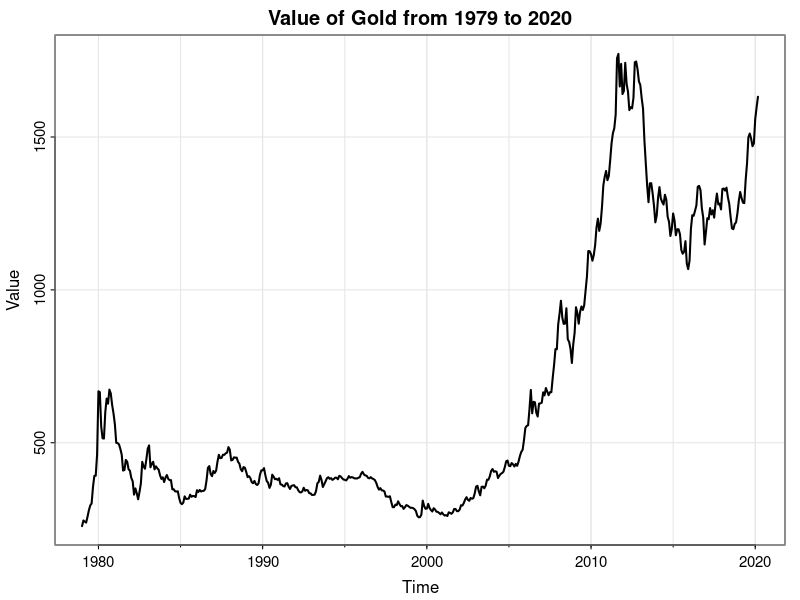
\includegraphics[width=1\textwidth]{images/data_plot.png}
    \caption{Value of gold from the first quarter of 1970 through the last quarter of 2020.}
    \label{fig:figure_1}
\end{figure}

We can see that the data is not stationary, since the mean and variance are not constant over time. In order to fit a time series model, we need to make the dataset stationary first. There are several techniques that can be used to achieve this. The most common technique is taking first order differencing. This technique involves computing the difference between consecutive observations in the series, effectively focusing on the changes between periods rather than the actual values themselves.
$$\Delta X_t = X_t - X_{t-1}$$

\begin{figure}[h]
    \centering
    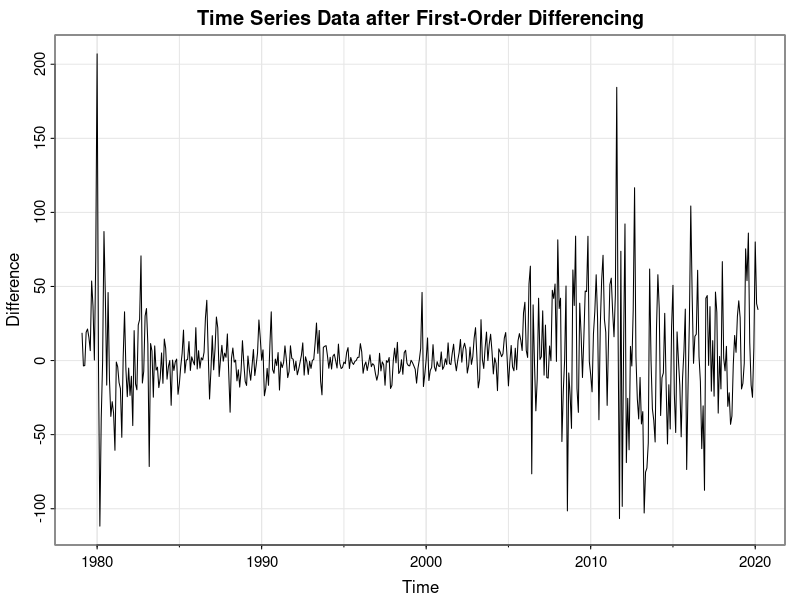
\includegraphics[width=1\textwidth]{images/diff_plot.png}
    \caption{Dataset after taking first-order differencing.}
    \label{fig:figure_2}
\end{figure}

\newpage
After differencing the dataset, it seems that we have achieved stationarity. The mean and variance seem to be constant over time with no extreme fluctuations. However, it is important to not only rely on visual inspection but also to perform statistical tests to confirm stationarity. One of the most common statistical tests for stationarity is the Augmented Dickey-Fuller (ADF) Test. 


$H_0$: Data is non-stationary.
$H_a$: Data is stationary.


% Please add the following required packages to your document preamble:
% \usepackage{graphicx}
% \usepackage[table,xcdraw]{xcolor}
% Beamer presentation requires \usepackage{colortbl} instead of \usepackage[table,xcdraw]{xcolor}
% \usepackage[normalem]{ulem}
% \useunder{\uline}{\ul}{}
\begin{table}[h]
\centering
\resizebox{0.6\columnwidth}{!}{%
\begin{tabular}{|lll|}
\hline
\rowcolor[HTML]{EFEFEF} 
\multicolumn{3}{|c|}{\cellcolor[HTML]{EFEFEF}{\ul \textbf{Dickey-Fuller Test Results}}}                                                                    \\ \hline
\rowcolor[HTML]{EFEFEF} 
\multicolumn{1}{|l|}{\cellcolor[HTML]{EFEFEF}\textbf{Test Statistic}} & \multicolumn{1}{l|}{\cellcolor[HTML]{EFEFEF}\textbf{Lag Order}} & \textbf{p-value} \\ \hline
\multicolumn{1}{|l|}{-7.0536}                                         & \multicolumn{1}{l|}{7}                                         & 0.01             \\ \hline
\end{tabular}%
}
\caption{Augmented Dickey-Fuller Test results on first-order differenced dataset.}
\label{tab:my-table}
\end{table}

With a test statistic of -7.0536 and a p-value of 0.01, we have strong evidence to reject the null hypothesis, indicating that the differenced dataset is stationary.

Next we will be plotting the Autocorrelation Function (ACF) and the Partial Autocorrelation Function (PACF) for our first-differenced dataset. This will guide us in selecting the most appropriate model for this dataset.

\begin{figure}[h]
    \centering
    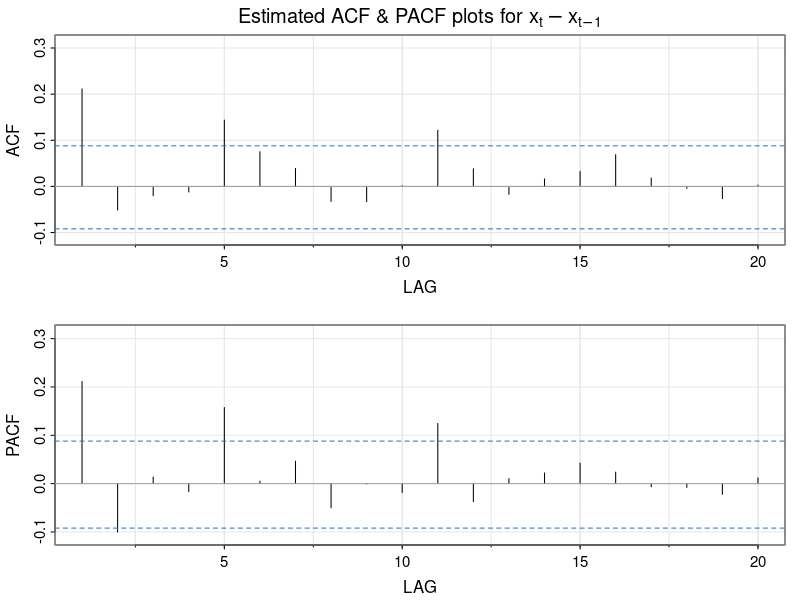
\includegraphics[width=1\textwidth]{images/acf_pacf_plot.png}
    \caption{ACF and PACF plot for the first-differenced dataset.}
    \label{fig:figure_3}
\end{figure}

These autocorrelation plots tell us the kind of models to choose from for the time series data. For the ACF plot, lag 1 is significant, suggesting that an MA(1) component might be significant for a future model. For the PACF plot, both lag 1 and 2 are significant, suggesting that AR(1) and AR(2) components could also be significant. Based on this, we can try a few different model combinations and compare their performance based on metrics such as the Bayesian Information Criterion (BIC) or, alternatively, the Akaike Information Criterion (AIC).

\section{Model Building}
At first we will start by incorporating AR components into the model, given we have significant correlations at lag 1 and 2 on the PACF plot. We will compare the components' significance levels and the distribution of the residuals.

\subsection{ARIMA(1,1,0)}
First we will build a model with just one AR component.

% latex table generated in R 4.3.2 by xtable 1.8-4 package
% Sat Mar 16 22:06:22 2024
\begin{table}[ht]
\centering
\begin{tabular}{rrrrr}
  \hline
 & Estimate & SE & t.value & p.value \\ 
  \hline
ar1 & 0.21 & 0.04 & 4.81 & 0.00 \\ 
  constant & 2.87 & 1.76 & 1.63 & 0.10 \\ 
   \hline
\end{tabular}
\caption{Model estimates for ARIMA(1,1,0) model.}
\end{table}
% latex table generated in R 4.3.2 by xtable 1.8-4 package
% Sat Mar 16 22:12:35 2024
\begin{table}[ht]
\centering
\begin{tabular}{rrrr}
  \hline
 & AIC & AICc & BIC \\ 
  \hline
Value & 9.713268 & 9.713318 & 9.738790 \\ 
   \hline
\end{tabular}
\caption{IC values for ARIMA(1,1,0) model.}
\end{table}
The p-value for the AR1 component is  $<$ 0.01. This low p-value suggests that there is statistically significant evidence that the first lag of the series has a linear predictive value for the series after differencing.

\begin{figure}[ht]
\centering

\begin{subfigure}[b]{0.6\textwidth}
\centering
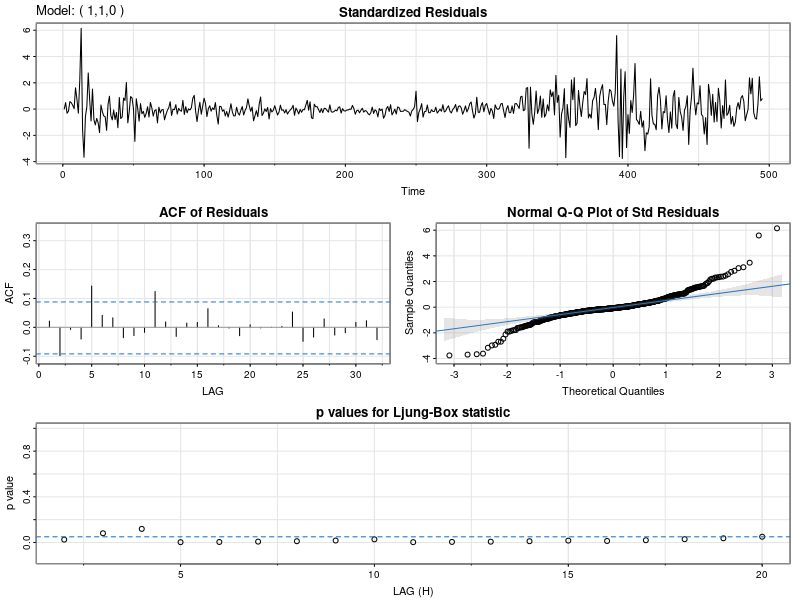
\includegraphics[width=1\textwidth]{images/arima_110.png}
\label{fig:sub1}
\end{subfigure}

\begin{subfigure}[b]{0.6\textwidth}
\centering
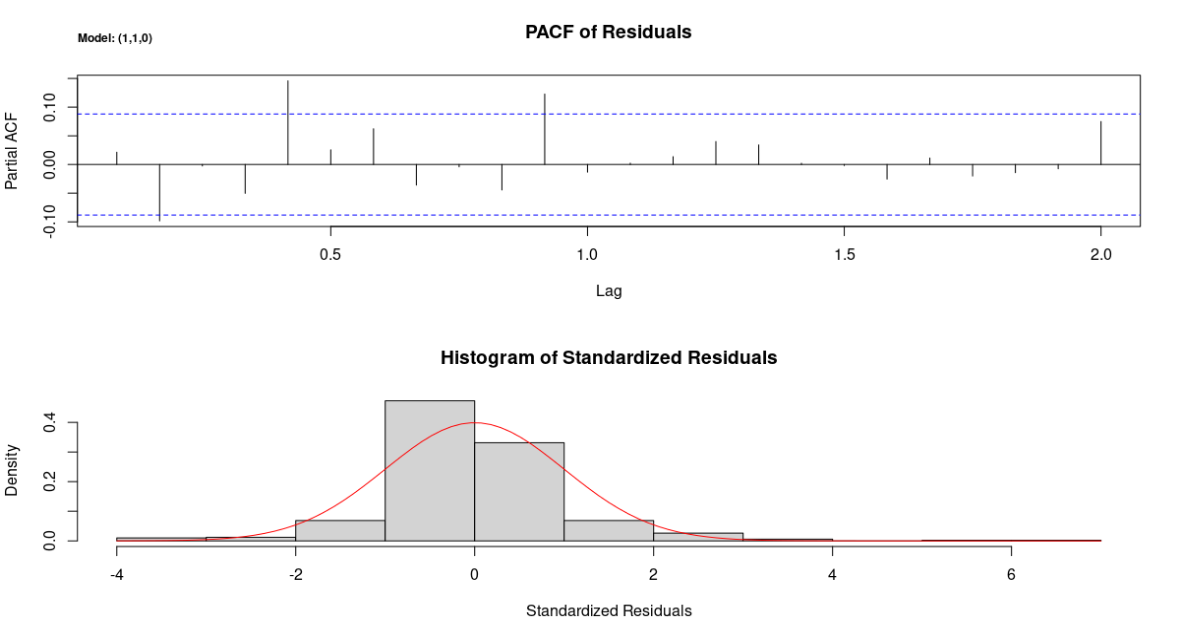
\includegraphics[width=1\textwidth]{images/arima_110_examine.png}
\label{fig:sub2}
\end{subfigure}

\caption{Model diagnostics for ARIMA(1,1,0).}
\label{fig:test}
\end{figure}


When looking at the diagnostic plot, we can see that the residual is not evenly spread without clear structure. The ACF of the residuals shows significant autocorrelation at different lags, which is confirmed by the Ljung-Box statistics at different lags. The normal QQ plot and the histogram also show that the residuals are not normally distributed. These results suggest that the ARIMA(1,1,0) model may not be the best fit for the data, and that a better model may exist.

\newpage

\subsection{ARIMA(2,1,0)}
Next, we will add an additional AR component and compare the results.

% latex table generated in R 4.3.2 by xtable 1.8-4 package
% Sat Mar 16 22:06:50 2024
\begin{table}[ht]
\centering
\begin{tabular}{rrrrr}
  \hline
 & Estimate & SE & t.value & p.value \\ 
  \hline
ar1 & 0.23 & 0.04 & 5.19 & 0.00 \\ 
  ar2 & -0.10 & 0.04 & -2.23 & 0.03 \\ 
  constant & 2.84 & 1.60 & 1.78 & 0.08 \\ 
   \hline
\end{tabular}
\caption{Model estimates for ARIMA(2,1,0) model.}
\end{table}
% latex table generated in R 4.3.2 by xtable 1.8-4 package
% Sat Mar 16 22:13:01 2024
\begin{table}[ht]
\centering
\begin{tabular}{rrrr}
  \hline
 & AIC & AICc & BIC \\ 
  \hline
Value & 9.707301 & 9.707400 & 9.741330 \\ 
   \hline
\end{tabular}
\caption{IC values for ARIMA(2,1,0) model.}
\end{table}
The p-value for the AR1 component is $<$ 0.01, and for the AR2 component it is 0.03. Since both AR components are statistically significant, this means that the additional component may improve upon our previous model.

\newpage

\begin{figure}[ht]
\centering

\begin{subfigure}[b]{0.6\textwidth}
\centering
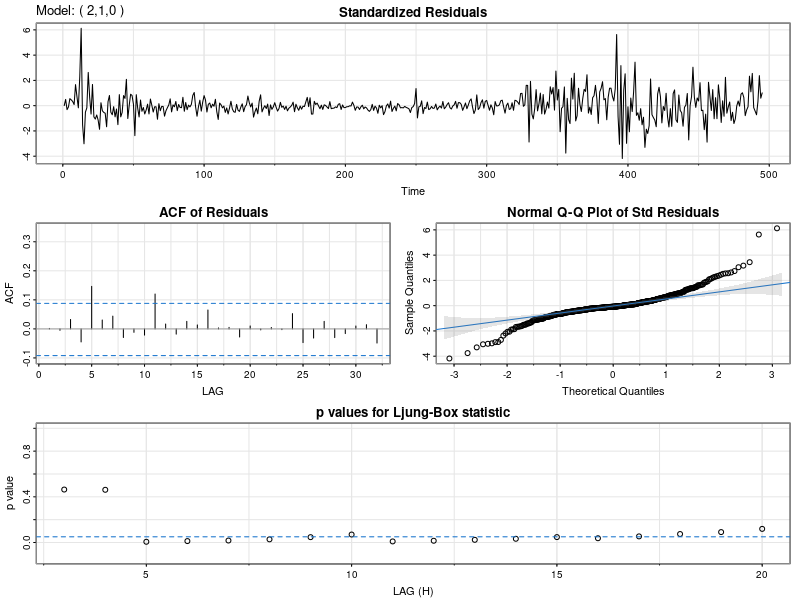
\includegraphics[width=1\textwidth]{images/arima_210.png}
\label{fig:sub1}
\end{subfigure}

\begin{subfigure}[b]{0.6\textwidth}
\centering
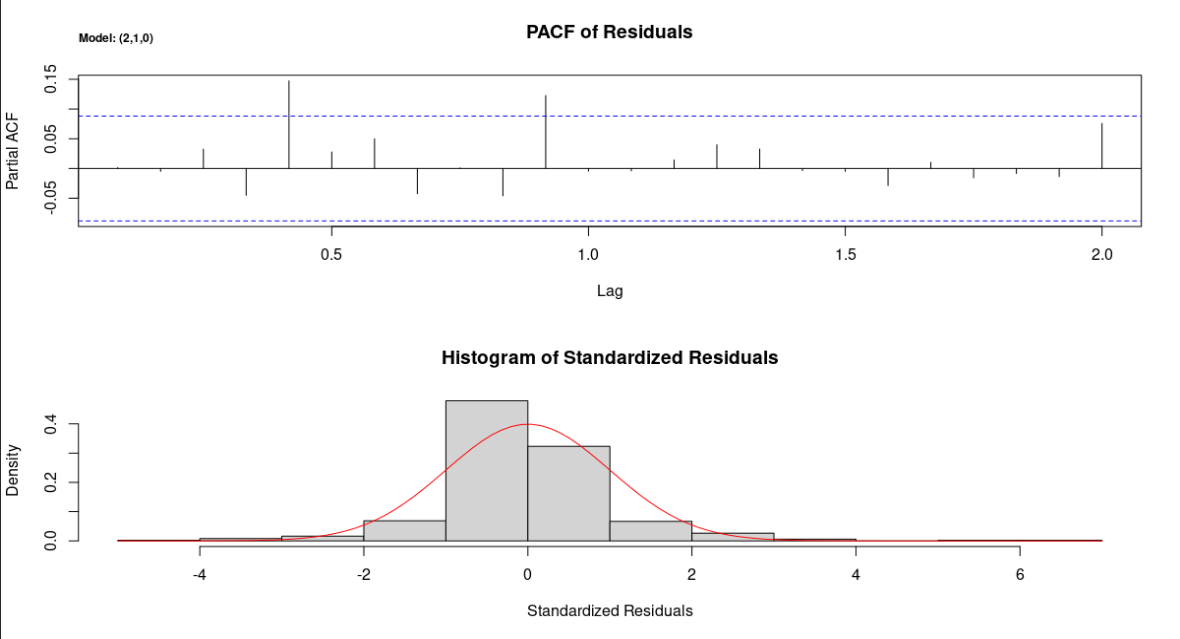
\includegraphics[width=1\textwidth]{images/arima_210_examine.png}
\label{fig:sub2}
\end{subfigure}

\caption{Model diagnostics for ARIMA(2,1,0).}
\label{fig:test}
\end{figure}
\newpage

The diagnostic plot for ARIMA(2,1,0) is similar to the previous one. Although the residual fluctuates around zero, there are still some periods of high volatility, particularly around 2008-2011.Looking at the ACF and PACF plots, there is autocorrelation present at different lags 5 and 11. The Ljung-Box plot confirms there is no significant autocorrelation for the first four lags. The normal QQ plot and the histogram also indicate that the residuals do not follow a normal distribution. These results suggest that the ARIMA(2,1,0) is an improvement upon our previous model and is more viable.

\newpage

\subsection{ARIMA(3,1,0)}
Since ARIMA(2,1,0) performed better compared to ARIMA(1,1,0), we will add an additional AR component and compare its performance with the aforementioned models.

% latex table generated in R 4.3.2 by xtable 1.8-4 package
% Sat Mar 16 22:07:05 2024
\begin{table}[ht]
\centering
\begin{tabular}{rrrrr}
  \hline
 & Estimate & SE & t.value & p.value \\ 
  \hline
ar1 & 0.23 & 0.04 & 5.20 & 0.00 \\ 
  ar2 & -0.10 & 0.05 & -2.24 & 0.03 \\ 
  ar3 & 0.01 & 0.05 & 0.31 & 0.75 \\ 
  constant & 2.85 & 1.62 & 1.76 & 0.08 \\ 
   \hline
\end{tabular}
\caption{Model estimates for ARIMA(3,1,0) model.}
\end{table}


% latex table generated in R 4.3.2 by xtable 1.8-4 package
% Sat Mar 16 22:13:21 2024
\begin{table}[ht]
\centering
\begin{tabular}{rrrr}
  \hline
 & AIC & AICc & BIC \\ 
  \hline
Value & 9.711151 & 9.711316 & 9.753686 \\ 
   \hline
\end{tabular}
\caption{IC values for ARIMA(3,1,0) model.}
\end{table}

As before, the first two AR components of the model are still statistically significant. The additional AR component of this model though is not, with a p-value of 0.75. This suggests that this model may be too complex with no additional signal provided.

\begin{figure}[h!]
\centering

\begin{subfigure}[b]{0.6\textwidth}
\centering
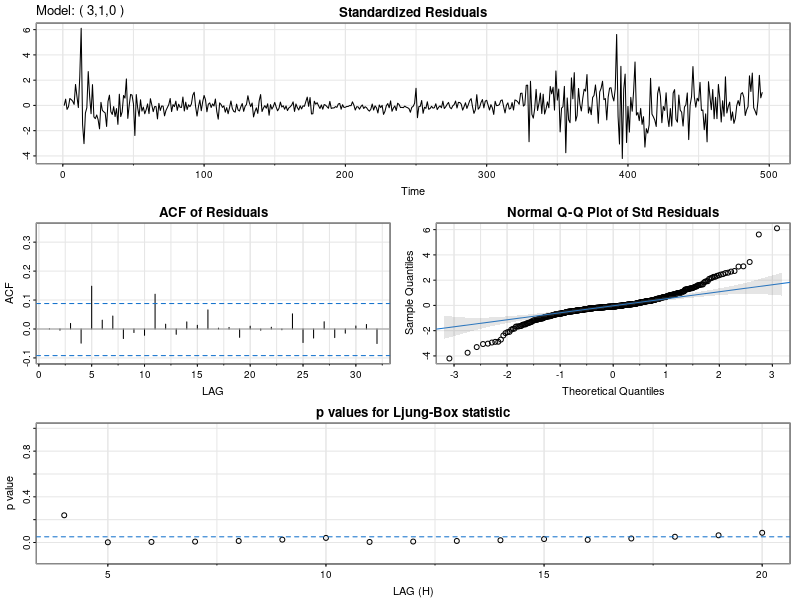
\includegraphics[width=1\textwidth]{images/arima_310.png}
\label{fig:sub1}
\end{subfigure}

\begin{subfigure}[b]{0.6\textwidth}
\centering
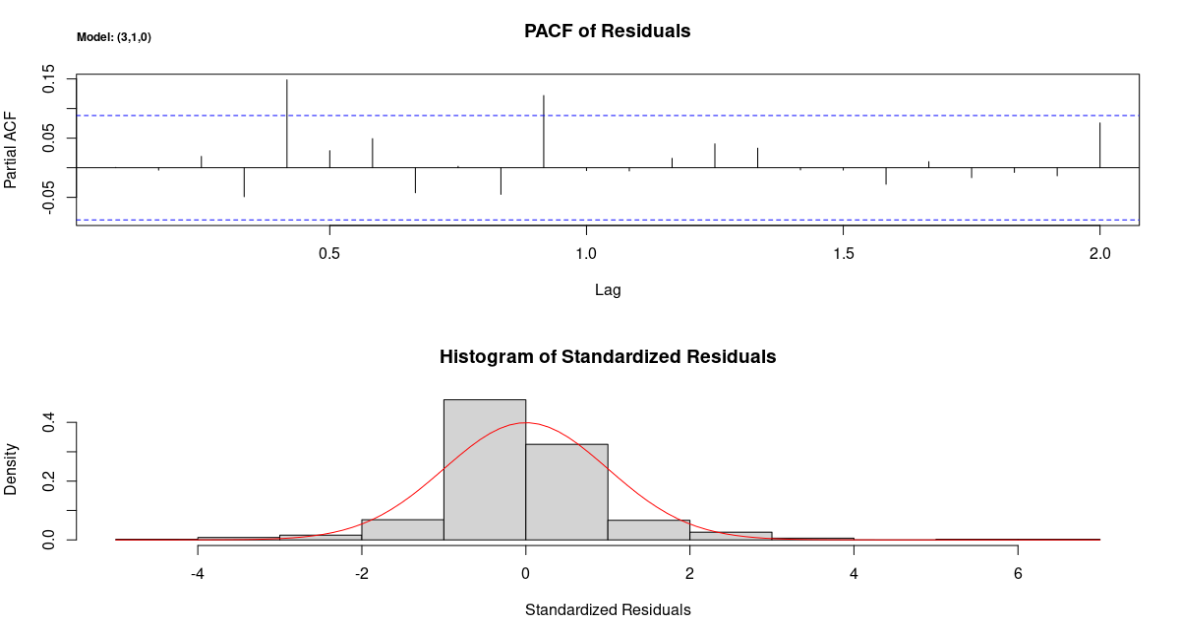
\includegraphics[width=1\textwidth]{images/arima_310_examine.png}
\label{fig:sub2}
\end{subfigure}

\caption{Model diagnostics for ARIMA(3,1,0).}
\label{fig:test}
\end{figure}



Looking at the diagnostic plots, this model performs very similarly to our previous model, with some autocorrelation present at lags 5 and 11 and outliers at each tail of the distribution. Since we already know that the AR(3) component is not statistically significant, we will reject this model for the simpler ARIMA(2,1,0) model up to this point.

\subsection{ARIMA(0,1,1)}
Next, we will start exploring some models that contain only moving average components and follow the same method of adding additional MA components depending on those components' significance.


% latex table generated in R 4.3.2 by xtable 1.8-4 package
% Sat Mar 16 22:07:20 2024
\begin{table}[ht]
\centering
\begin{tabular}{rrrrr}
  \hline
 & Estimate & SE & t.value & p.value \\ 
  \hline
ma1 & 0.25 & 0.05 & 5.35 & 0.00 \\ 
  constant & 2.86 & 1.73 & 1.65 & 0.10 \\ 
   \hline
\end{tabular}
\caption{Model estimates for ARIMA(0,1,1) model.}
\end{table}
% latex table generated in R 4.3.2 by xtable 1.8-4 package
% Sat Mar 16 22:13:35 2024
\begin{table}[ht]
\centering
\begin{tabular}{rrrr}
  \hline
 & AIC & AICc & BIC \\ 
  \hline
Value & 9.704995 & 9.705045 & 9.730517 \\ 
   \hline
\end{tabular}
\caption{IC values for ARIMA(0,1,1) model.}
\end{table}
The p-value for the MA1 component is $<$ 0.01, which is below our significance level. This suggests that the error term from the previous time step provides valuable information in predicting the current step's value after differencing.

\begin{figure}[h!]
\centering

\begin{subfigure}[b]{0.6\textwidth}
\centering
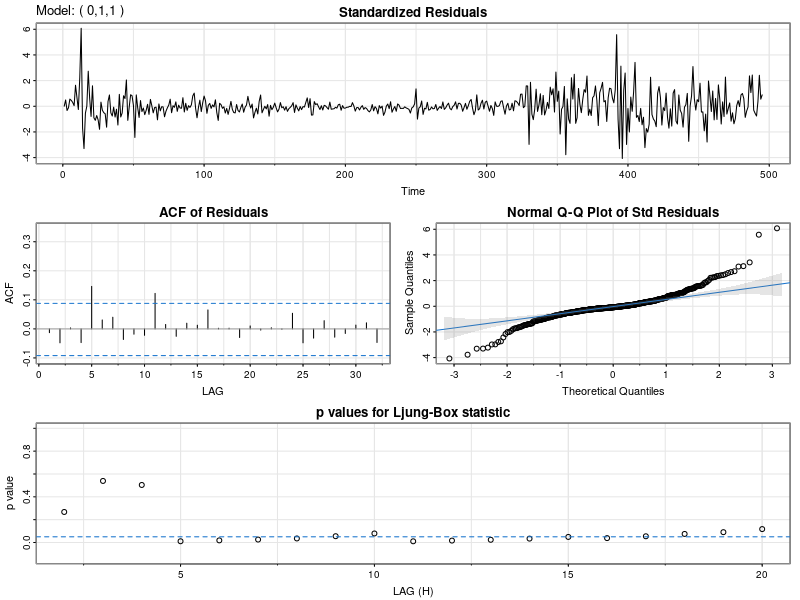
\includegraphics[width=1\textwidth]{images/arima_011.png}
\label{fig:sub1}
\end{subfigure}

\begin{subfigure}[b]{0.6\textwidth}
\centering
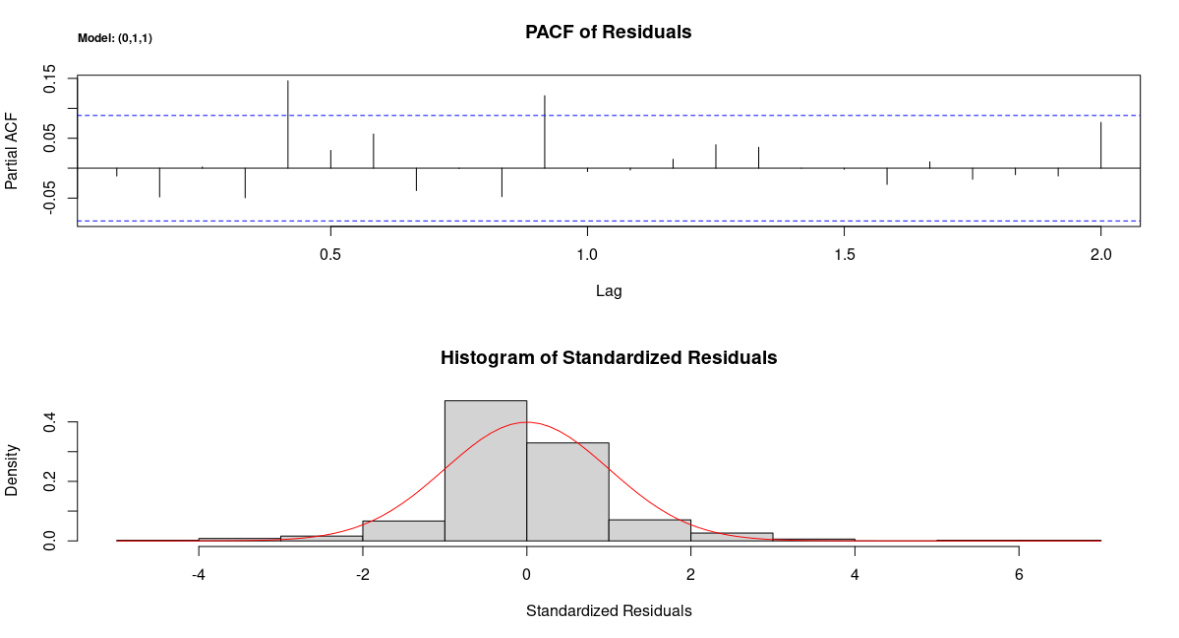
\includegraphics[width=1\textwidth]{images/arima_011_examine.png}
\label{fig:sub2}
\end{subfigure}

\caption{Model diagnostics for ARIMA(0,1,1).}
\label{fig:test}
\end{figure}

The distribution of the residuals is very similar to our previous autoregressive models, There seems to be some volatility at the starting and ending points of the time series, with the same autocorrelated lag points present on the ACF and PACF plots. The distribution of the residuals has outliers present at both tails of the distribution. The Ljung-Box plot has an addidional non-significant autocorrelation lag, suggesting that the MA model is a viable option, especially as we further explore additional moving average parts and combinations of autoregressive and moving average.
\newpage
\section{ARIMA(0,1,2)}
Next, we will add an additional MA component model to compare its performance to the previous moving average model.

% latex table generated in R 4.3.2 by xtable 1.8-4 package
% Sat Mar 16 22:07:37 2024
\begin{table}[ht]
\centering
\begin{tabular}{rrrrr}
  \hline
 & Estimate & SE & t.value & p.value \\ 
  \hline
ma1 & 0.24 & 0.04 & 5.31 & 0.00 \\ 
  ma2 & -0.07 & 0.05 & -1.34 & 0.18 \\ 
  constant & 2.85 & 1.62 & 1.76 & 0.08 \\ 
   \hline
\end{tabular}
\caption{Model estimates for ARIMA(0,1,2) model.}
\end{table}
% latex table generated in R 4.3.2 by xtable 1.8-4 package
% Sat Mar 16 22:13:59 2024
\begin{table}[ht]
\centering
\begin{tabular}{rrrr}
  \hline
 & AIC & AICc & BIC \\ 
  \hline
Value & 9.705457 & 9.705557 & 9.739486 \\ 
   \hline
\end{tabular}
\caption{IC values for ARIMA(0,1,2) model.}
\end{table}

The p-value for the MA1 component is still $<$ 0.01, but the MA2 component is not statistically significant. The diagnostics plot for ARIMA(0,1,2) is very similar to the ones from ARIMA(0,1,1), but the additional complexity added by the second moving average component is not justified based on its significance.


\begin{figure}[h!]
\centering

\begin{subfigure}[b]{0.6\textwidth}
\centering
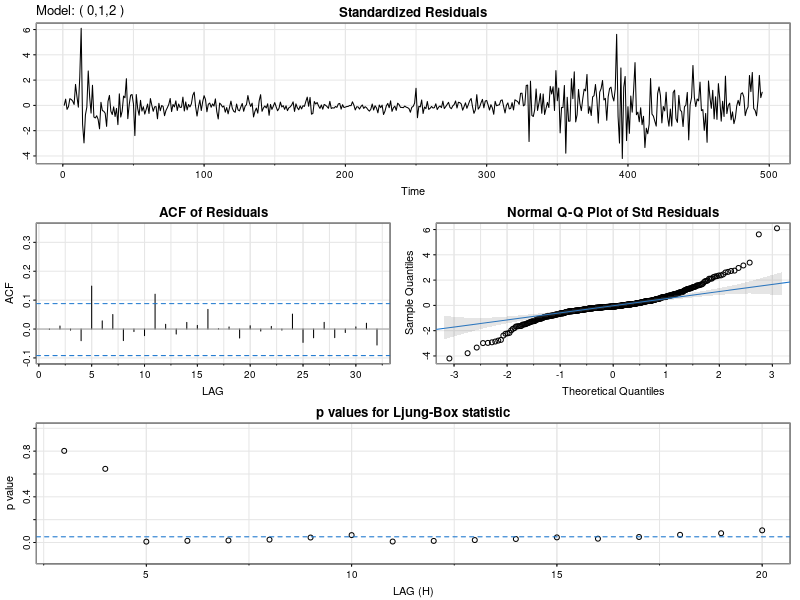
\includegraphics[width=1\textwidth]{images/arima_012.png}
\label{fig:sub1}
\end{subfigure}

\begin{subfigure}[b]{0.6\textwidth}
\centering
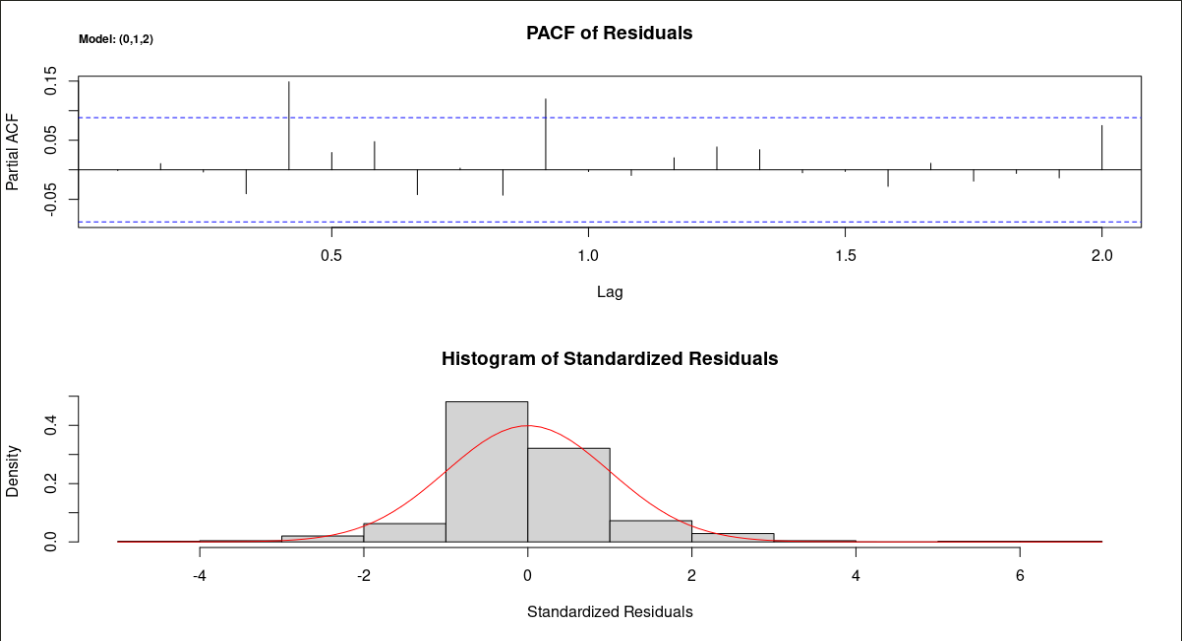
\includegraphics[width=1\textwidth]{images/arima_012_examine.png}
\label{fig:sub2}
\end{subfigure}

\caption{Model diagnostics for ARIMA(0,1,2).}
\label{fig:test}
\end{figure}

\section{ARIMA(2,1,1)}
Since our previous model fits have shown that ARIMA(2,1,0) and ARIMA(0,1,1) both contained statistically significant components, we can explore a synthesis of the two modelsby testing an ARIMA(2,1,1) model. 

% latex table generated in R 4.3.2 by xtable 1.8-4 package
% Sat Mar 16 22:07:53 2024
\begin{table}[ht]
\centering
\begin{tabular}{rrrrr}
  \hline
 & Estimate & SE & t.value & p.value \\ 
  \hline
ar1 & -0.61 & 0.08 & -7.79 & 0.00 \\ 
  ar2 & 0.10 & 0.05 & 1.85 & 0.06 \\ 
  ma1 & 0.86 & 0.06 & 13.69 & 0.00 \\ 
  constant & 2.86 & 1.69 & 1.70 & 0.09 \\ 
   \hline
\end{tabular}
\caption{Model estimates for ARIMA(2,1,1) model.}
\end{table}
% latex table generated in R 4.3.2 by xtable 1.8-4 package
% Sat Mar 16 22:14:14 2024
\begin{table}[ht]
\centering
\begin{tabular}{rrrr}
  \hline
 & AIC & AICc & BIC \\ 
  \hline
Value & 9.697469 & 9.697634 & 9.740004 \\ 
   \hline
\end{tabular}
\caption{IC values for ARIMA(2,1,1) model.}
\end{table}

The p-values for the AR1 and MA1 components are both statistically significant. For the AR2 component though, the p-value is 0.06, which is right above our predetermined significance level. This borderline p-value places us in a grey area of statistical inference, where the decision to include or exclude the AR2 term from the model may depend on additional considerations beyond the p-value alone.


\begin{figure}[h!]
\centering

\begin{subfigure}[b]{0.6\textwidth}
\centering
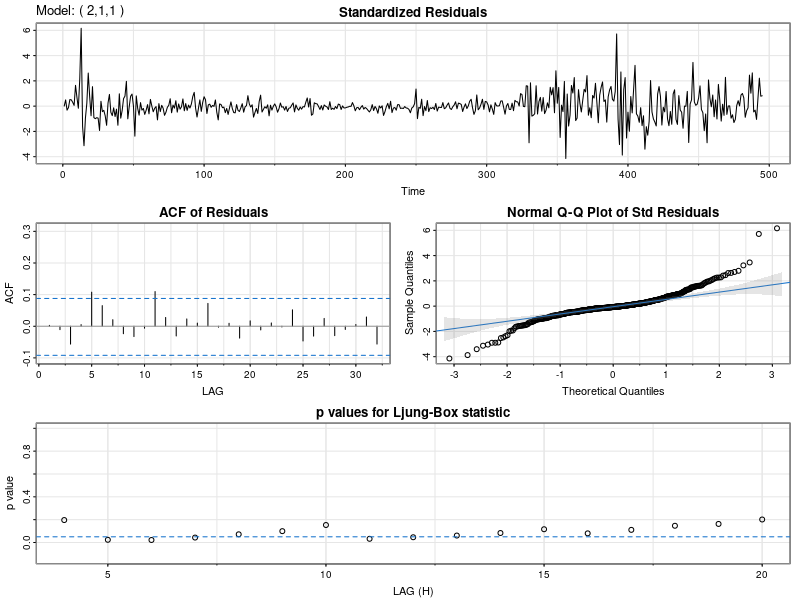
\includegraphics[width=1\textwidth]{images/arima_211.png}
\label{fig:sub1}
\end{subfigure}

\begin{subfigure}[b]{0.6\textwidth}
\centering
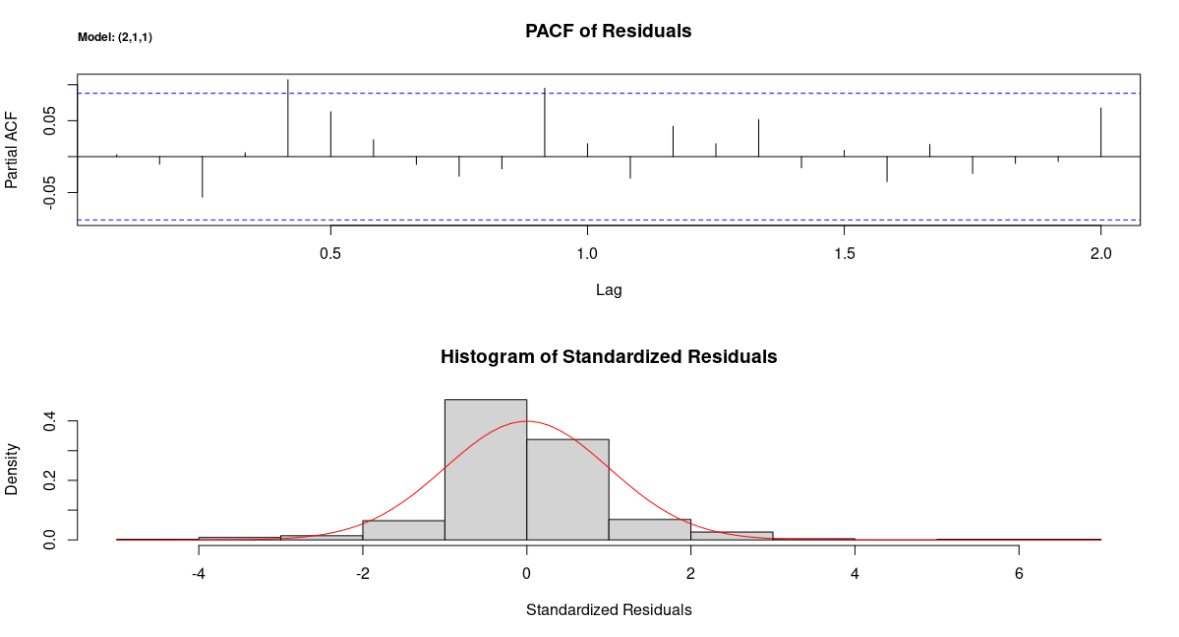
\includegraphics[width=1\textwidth]{images/arima_211_examine.png}
\label{fig:sub2}
\end{subfigure}

\caption{Model diagnostics for ARIMA(2,1,1).}
\label{fig:test}
\end{figure}
\newpage
\section{Model Comparison}
After having fit multiple models, we will compare and evaluate them using their AIC and BIC scores. These metrics are statistical measures used to compare the goodness of fit of different models and penalize overly-complex models. They will help us discern which model has the optimal balance between accuracy and complexity.
\begin{itemize}
  \item AIC (Akaike Information Criterion) = $2k - 2ln(L)$, where $k$ is the number of parameters and L the likelihood of the model given the data.
  \item AICc = Adds an additional penalty for models with more parameters when the sample size is small, making it less likely to select overfitted models. 
  \item BIC (Bayesian Information Criterion) = $kln(n) - 2ln(L)$
\end{itemize}

% latex table generated in R 4.3.2 by xtable 1.8-4 package
% Sun Mar 17 17:41:10 2024
\begin{table}[ht]
\centering
\begin{tabular}{rlrrr}
  \hline
 & Model & AIC & AICc & BIC \\ 
  \hline
1 & ARIMA(1,1,0) & 9.713268 & 9.713318 & 9.738790 \\ 
  2 & ARIMA(2,1,0) & 9.707301 & 9.707400 & 9.741330 \\ 
  3 & ARIMA(3,1,0) & 9.711151 & 9.711316 & 9.753686 \\ 
  4 & ARIMA(0,1,1) & 9.704995 & 9.705045 & 9.730517 \\ 
  5 & ARIMA(0,1,2) & 9.705457 & 9.705557 & 9.739486 \\ 
  6 & ARIMA(2,1,1) & 9.697469 & 9.697634 & 9.740004 \\ 
   \hline
\end{tabular}
\caption{IC results for all fitted models.}
\end{table}

The model with the lowest AIC value is ARIMA(2,1,1) and the model with the lowest BIC value is ARIMA(0,1,1). Since AIC is more focused on the predictive accuracy of a model, we will choose ARIMA(2,1,1) as our final model and perform forecasting.

\section{Forecasting Future Values}
In this section, we will be forecasting future values using the ARIMA(2,1,1) model, which has been identified as the most suitable model based on its relative performance compared to the other models.
$$\textbf{ARIMA(2,1,1)}: (1+ 0.6148B - 0.0983B^2)(1-B)X_t = (1-0.8636B)w_t + 2.8634$$

\begin{figure}
    \centering
    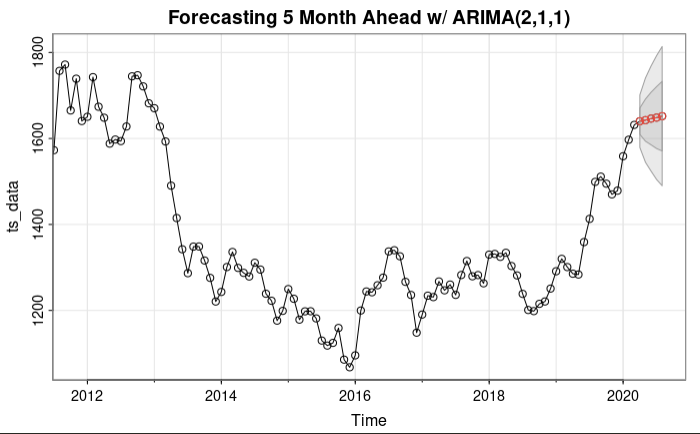
\includegraphics[width=1\textwidth]{images/forecast.png}
    \caption{ARIMA(2,1,1) forecasting for the next 5 months.}
    \label{fig:enter-label}
\end{figure}

From the plot we can see that the model seems to be picking up a continuation of the recent increasing trend observed in the historical data. This suggests that the model expects the increasing trend will continue into the future. The confidence interval for our predictions is quite wide, accounting for any uncertainty in our predicted values. 

We can also plot our observed and predicted values for all of the time points in the dataset and compare how closely they match.

\begin{figure}
    \centering
    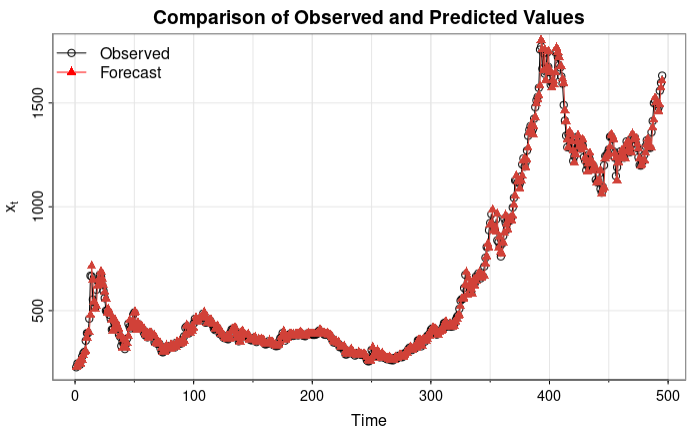
\includegraphics[width=1\textwidth]{images/observed_predicted.png}
    \caption{}
    \label{fig:enter-label}
\end{figure}

We can see from the plot that the forecasted values track closely with the observed data, suggesting that the ARIMA(2,1,1) model is capturing the underlying trend of the series well.

\section{Final Discussion}
Throughout our investigation, we have applied various time series models with the goal of uncovering the nuanced patterns that have affected goal prices from 1979 to 2020. After applying and testing multiple models, we arrived at the ARIMA(2,1,1) model. which demonstrated the strongest capacity of capturing the underlying trends present in the dataset. However, it is important to keep in mind the limitations of the current model in regards to gold price predictions. Despite our model's predictive performance, gold market prices tend to fluctuate and are highly sensitive to global economic conditions. A more accurate model would perhaps take into account additional indicators other than prices at previous time points, but such a model at this time is outside the scope of this project.

\bibliographystyle{apalike}
\bibliography{bibliography}

\appendix
\section*{Appendix}
\section{R Code for ARIMA Model Fitting and Diagnostics}
\begin{lstlisting}[language=R]
    # Load required libraries
    library(astsa)
    library(tseries)
    library(forecast)
    library(dplyr)
    library(zoo)
    library(ggplot2)
    library(xtable)
\end{lstlisting}

\begin{lstlisting}[language=R]
    # Load the dataset
    df <- read.csv('gold_price_data.csv')
    df$Date <- as.POSIXct(df$Date)
    head(df)
\end{lstlisting}

\begin{lstlisting}
    # Remove data prior to 1979 
    cutoff_date <- as.Date("1979-01-01")
    df2 <- df %>% filter(Date >= cutoff_date)
    head(df2)
    
    # Create zoo object
    zoo_data <- zoo(df2$Value, order.by=df2$Date)
    # Aggregate data monthly
    monthly_data <- aggregate(zoo_data, as.yearmon, mean)  # Replace 'mean' with your function
    
    # Convert back to dataframe
    monthly_df <- data.frame(date = index(monthly_data), value = coredata(monthly_data))
    monthly_df

    # Create time series object
    ts_data <- ts(monthly_df$value, frequency=12, start=c(1979,1))
    head(ts_data)
\end{lstlisting}

\begin{lstlisting}
    # Plot the data
    png("data_plot.png", width=800, height=600, res=100)
    tsplot(ts_data, main="Value of Gold from 1979 to 2020", xlab='Time', ylab='Value', lw=2)
    axis.POSIXct(1, at=seq(from=min(df$Date), to=max(df$Date), by="5 years"), format="%Y")
    dev.off()
\end{lstlisting}

\begin{lstlisting}
    # Take first-order differencing to achieve stationarity
    diff_x <-diff(ts_data,differences = 1)
    head(diff_x)
              Feb       Mar       Apr       May       Jun       Jul
1979 18.454783 -3.622273 -3.383442 19.118323 21.284058 15.669697
\end{lstlisting}

\begin{lstlisting}
    # Plot the data after differencing
    png("diff_plot.png", width=800, height=600, res=100)
    tsplot(diff_x, main="Time Series Data after First-Order Differencing", xlab="Time", ylab="Difference")
    dev.off()
\end{lstlisting}

\begin{lstlisting}
    # Perform augmented Dickey-Fuller Test to check stationarity
    adf.test(diff_x)
    Warning: p-value smaller than printed p-value
    Augmented Dickey-Fuller Test
    data:  diff_x
    Dickey-Fuller = -7.0536, Lag order = 7, p-value = 0.01
    alternative hypothesis: stationary
\end{lstlisting}

\begin{lstlisting}
    # ACF and PACF plots
    png("acf_pacf_plot.png", width=800, height=600, res=100)
    astsa::acf2(as.numeric(diff_x), max.lag=20, main=expression(paste("Estimated ACF & PACF plots for ", x[t] - x[t-1])))
    dev.off()
\end{lstlisting}

\begin{lstlisting}
    # ARIMA(1,1,0) Model
    png('arima_110.png', width=800, height=600, res=100)
    arima.110 <- sarima(as.numeric(ts_data), p=1, d=1, q=0)
    dev.off()

    examine.mod(arima.110, 1, 1, 0)
\end{lstlisting}

\begin{lstlisting}
    # ARIMA(2,1,0)
    png('arima_210.png', width=800, height=600, res=100)
    arima.210 <- sarima(as.numeric(ts_data), p=2, d=1, q=0)
    dev.off()

    examine.mod(arima.210, 2, 1, 0)
\end{lstlisting}

\begin{lstlisting}
    # ARIMA(3,1,0)
    png('arima_310.png', width=800, height=600, res=100)
    arima.310 <- sarima(as.numeric(ts_data), p=3, d=1, q=0)
    dev.off()
    
    examine.mod(arima.310, 3, 1, 0)
\end{lstlisting}

\begin{lstlisting}
    ### ARIMA(0,1,1)
    png('arima_011.png', width=800, height=600, res=100)
    arima.011 <- sarima(as.numeric(ts_data), p=0, d=1, q=1)
    dev.off()
    
    examine.mod(arima.011, 0, 1, 1)
\end{lstlisting}

\begin{lstlisting}
    # ARIMA(0,1,2)
    png('arima_012.png', width=800, height=600, res=100)
    arima.012 <- sarima(as.numeric(ts_data), p=0, d=1, q=2)
    dev.off()
    
    examine.mod(arima.012, 0, 1, 2)
\end{lstlisting}

\begin{lstlisting}
    # ARIMA(2,1,1)
    png('arima_211.png', width=800, height=600, res=100)
    arima.211 <- sarima(as.numeric(ts_data), p=2, d=1, q=1)
    dev.off()
    
    examine.mod(arima.211, 2, 1, 1)
\end{lstlisting}

\begin{lstlisting}
    # ARIMA(1,1,1)
    png('arima_111.png', width=800, height=600, res=100)
    arima.111 <- sarima(as.numeric(ts_data), p=1, d=1, q=1)
    dev.off()
    
    examine.mod(arima.111, 1, 1, 1)
\end{lstlisting}

\begin{lstlisting}
    # IC Results for all models
    data.frame(Model=c("ARIMA(1,1,0)", "ARIMA(2,1,0)", "ARIMA(3,1,0)", "ARIMA(0,1,1)", "ARIMA(0,1,2)", "ARIMA(2,1,1)", "ARIMA(1,1,1)"), 
           AIC=c(arima.110$ICs[1], arima.210$ICs[1], arima.310$ICs[1], arima.011$ICs[1], arima.012$ICs[1], arima.211$ICs[1], arima.111$ICs[1]),
           AICc=c(arima.110$ICs[2], arima.210$ICs[2], arima.310$ICs[2], arima.011$ICs[2], arima.012$ICs[2], arima.211$ICs[2], arima.111$ICs[2]),
           BIC=c(arima.110$ICs[3], arima.210$ICs[3], arima.310$ICs[3], arima.011$ICs[3], arima.012$ICs[3], arima.211$ICs[3], arima.111$ICs[3]))
\end{lstlisting}

\begin{lstlisting}
    # Forecast future values
    forecast <- sarima.for(ts_data, n.ahead=5, p=2, d=1, q=1, main='Forecasting 5 Month Ahead w/ ARIMA(2,1,1)')
    forecast
\end{lstlisting}

\begin{lstlisting}
    # Compare actual vs. predicted
    pred_x <- as.numeric(ts_data) - resid(arima.211$fit)
    tsplot(as.numeric(ts_data), ylab=expression(x[t]), type="o", main="Comparison of Observed and Predicted Values")
    lines(pred_x, col="#D14138", type="o", pch=17, lw=1) 
    legend("topleft", legend=c("Observed", "Forecast"), lty=c("solid", "solid"), col=c("black", "red"), pch=c(1, 17), bty="n")
\end{lstlisting}


\end{document}
